\documentclass[handout]{beamer}
% \documentclass{beamer}

%%
%%
%%
% From http://tex.stackexchange.com/questions/2072/beamer-navigation-circles-without-subsections
% Solution #2 or 3:
% \usepackage{etoolbox}
% \makeatletter
% % replace the subsection number test with a test that always returns true
% \patchcmd{\slideentry}{\ifnum#2>0}{\ifnum2>0}{}{\@error{unable to patch}}%
% \makeatother
% Solution #1:
\usepackage{remreset}% tiny package containing just the \@removefromreset command
\makeatletter
%\@removefromreset{subsection}{section}
%\makeatother
%\setcounter{subsection}{1}




\usepackage{etex}
\usepackage{pgf}
\usepackage{tikz}
\usepackage{url}
\usepackage{amsmath}
\usepackage{color}
% \definecolor{red}{rgb}{1,0,0}
\usepackage{ulem}
% \usepackage{booktabs}
\usepackage{colortbl,booktabs}
\renewcommand*{\thefootnote}{\fnsymbol{footnote}}
\usepackage{fancybox}
\usepackage[framemethod=TikZ]{mdframed}
\mdfdefinestyle{FactStyle}{%
  outerlinewidth=0.5,
  roundcorner=1pt,
  leftmargin=1cm,
  linecolor=blue,
  outerlinecolor=blue!70!black,
  backgroundcolor=yellow!40
}
\usepackage{cancel}

  \newcommand\Warning{%
    \makebox[2.4em][c]{%
      \makebox[0pt][c]{\raisebox{.2em}{\Large!}}%
      \makebox[0pt][c]{\color{red}\Huge$\bigtriangleup$}}}%

\usepackage{stackengine}
\usepackage{scalerel}
\usepackage{xcolor}
  \newcommand\dangersign[1][2ex]{%
    \renewcommand\stacktype{L}%
    \scaleto{\stackon[1.3pt]{\color{red}$\triangle$}{\tiny !}}{#1}%
  }



\usepackage{dcolumn}
\newcolumntype{d}[1]{D{.}{.}{#1}}

% From
% http://tex.stackexchange.com/questions/109900/how-can-i-box-multiple-aligned-equations
\usepackage{empheq}
\usepackage{tcolorbox}  \newtcbox{\othermathbox}[1][]{%
  nobeforeafter, tcbox raise base, 
  colback=black!10, colframe=red!30, 
  left=1em, top=0.5em, right=1em, bottom=0.5em}

\newcommand\blue{\color{blue}}
\newcommand\red{\color{red}}
\newcommand\green{\color{green!75!black}}
\newcommand\purple{\color{purple}}
\newcommand\bluegreen{\color{blue!75!green}}
\newcommand\orange{\color{orange}}
\newcommand\redgreen{\color{red!50!green}}
\newcommand\grey{\color{black}}
\newcommand\gap{\vspace{.1in}}
\newcommand\nb{${\red\bullet}\ $}
\newcommand\halfgap{\vspace{.05in}}
\newcommand\divideline{\line(1,0){352}}
\usepackage{marvosym} % for \Smiley

\newcommand{\bluealert}[1]{{\blue\textbf{#1}}}

% \usepackage{beamerthemesplit} %Key package for beamer
\usetheme{Singapore}
% \usetheme{Szeged}
% \usetheme{Garfield}
% \usetheme{CambridgeUS}
% \usenavigationsymbolstemplate{} %Gets rid of slide navigation symbols


\setbeamercolor{separation line}{use=structure,bg=structure.fg!50!bg}
% \begin{beamercolorbox}[colsep=0.5pt]
%   {upper separation line foot}
% \end{beamercolorbox}



\makeatletter
\setbeamertemplate{footline}
{
  \leavevmode%
  \hbox{%
% \begin{beamercolorbox}[colsep=0.5pt]
%   {upper separation line foot}
% \end{beamercolorbox}


  \begin{beamercolorbox}[wd=.5\paperwidth,ht=2.25ex,dp=2ex,colsep=0.5pt]%
    {upper separation line foot}
    \usebeamerfont{author in head/foot}%
    \hspace*{2ex}\insertshortdate:\ \insertshorttitle
  \end{beamercolorbox}%
  \begin{beamercolorbox}[wd=.5\paperwidth,ht=2.25ex,dp=2ex,right]{title in head/foot}%
    \usebeamerfont{title in head/foot}
    {\insertshortauthor}\hspace*{2ex}
  \end{beamercolorbox}}%
  % \begin{beamercolorbox}[wd=.333333\paperwidth,ht=2.25ex,dp=2ex,right]{date in head/foot}%
  %   \usebeamerfont{date in head/foot}\insertshortdate{}\hspace*{2em}
  %   \insertframenumber{} / \inserttotalframenumber\hspace*{2ex} 
  % \end{beamercolorbox}%
  \vskip0pt%
}
\makeatother

\usetikzlibrary{decorations.markings}
\usetikzlibrary{arrows}


\title{Final Exam Review}
\author{Schley, UCSB Mathematics}
\date{March 15, 2017}
%\institute{}


\useinnertheme{default}

\usefonttheme{serif}
% \usecolortheme{rose}
% \usecolortheme{whale}
% \usecolortheme{orchid}
\usecolortheme{crane}
% \usecolortheme{dolphin}


%TEMPLATE
\setbeamertemplate{navigation symbols}{}

\setbeamertemplate{note page}[compress]

\setbeamertemplate{frametitle}{
  \vspace{0.5em}
  % \begin{centering}
  {\huge\blue\textbf{\textmd{\insertframetitle}}}
  \par
  % \end{centering}
}

% From http://tex.stackexchange.com/questions/7032/good-way-to-make-textcircled-numbers:
\newcommand*\circled[1]{\tikz[baseline=(char.base)]{\node[shape=circle,draw,fill=orange,inner sep=1pt] (char) {#1};}} 
% \renewcommand{\labelenumi}{\circled{\textbf{\arabic{enumi}}}}

\let\olddescription\description
\let\oldenddescription\enddescription
\usepackage{enumitem}
\let\description\olddescription
\let\enddescription\oldenddescription

% \usepackage[loadonly]{enumitem}
\setlist[enumerate,1]{label=\colorbox{orange}{\arabic*.},font=\bfseries}
%\setlist[enumerate,2]{label=\colorbox{blue!25}{(\alph*)},font=\bfseries}
% \setlist[enumerate,1]{label=\arabic*.,font=\bfseries}
\setlist[itemize,1]{label=\red$\bullet$}
\setlist[itemize,2]{label=\blue$\bullet$}

\newcommand\answer[1]{\fbox{#1}}
% \renewcommand\answer[1]{}

\newcommand{\antilog}{\operatorname{antilog}}

\newcommand{\instructor}{Nathan Schley ({\it Sh}+{\it lye})}
\newcommand{\officehours}{T R 11-11:50, T 3:45-4:35 Details on Gauchospace.}
\newcommand{\email}{schley@math.ucsb.edu}
\newcommand{\officeloc}{South Hall 6701}
\newcommand{\copyrightinfo}{2022\ Daryl Cooper, Peter M.\ Garfield, Ebrahim Ebrahim \& Nathan Schley}
    













\title{}
\title{The Tangent Line Approximation}
\date{May 17, 2017}


\begin{document}
\small

\section*{Administration}

\frame{
  \frametitle{Office Hours!}
  % \ \vspace*{0.25in}

  {\Large{}Instructor:}\\
  \ \hspace*{0.2in} Peter M.\ Garfield, \url{garfield@math.ucsb.edu}\\[0.25em]

  {\Large{}Office Hours:}\\
  \ \hspace*{0.2in} Mondays 2--3\textsc{pm}\\
  \ \hspace*{0.2in} Tuesdays 10:30--11:30\textsc{am}\\
  \ \hspace*{0.2in} Thursdays 1--2\textsc{pm}\\
  \ \hspace*{0.2in} or by appointment \\[0.25em]

  {\Large{}Office:}\\
  \ \hspace*{0.2in} South Hall 6510\\[0.5em]

  \copyright\ 2017\ Daryl Cooper, Peter M.\ Garfield

  % \vspace*{2in}
}

\frame{

  \begin{center}
    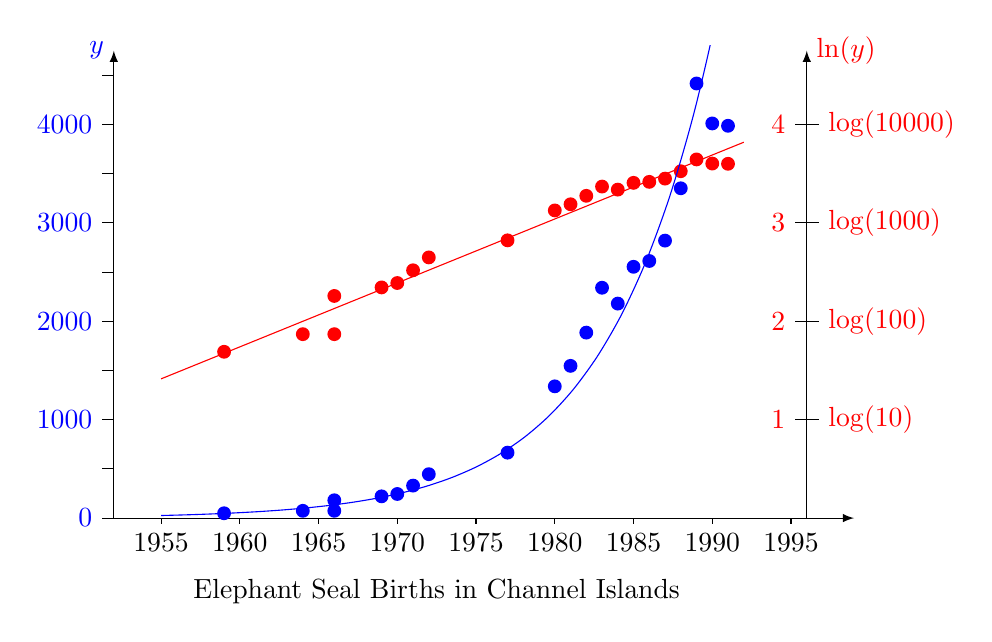
\begin{tikzpicture}[x=2mm,y=0.0125mm,>=latex]
      \draw[thin,black,->] (52,0) -- (99,0);
      \draw[thin,black,->] (52,0) -- (52,4750) node[left,blue] {$y$};
      % ticks:
      \foreach \k in {55,60,...,95}
      {
        \draw[thin,black] (\k,0) -- (\k,-2pt) node[below] {$19\k$};
      }
      \foreach \y in {0,1000,...,4000}
      {
        \draw[thin,black] (52,\y) -- (51.25,\y) node[left,blue] {$\y$};
      }
      \foreach \y in {500,1500,...,4500}
      {
        \draw[thin,black] (52,\y) -- (51.25,\y);
      }
      \fill[blue] (59,49) circle (2.5pt);
      \fill[blue] (64,74) circle (2.5pt);
      \fill[blue] (66,74) circle (2.5pt);
      \fill[blue] (66,181) circle (2.5pt);
      \fill[blue] (69,221) circle (2.5pt);
      \fill[blue] (70,245) circle (2.5pt);
      \fill[blue] (71,330) circle (2.5pt);
      \fill[blue] (72,446) circle (2.5pt);
      \fill[blue] (77,665) circle (2.5pt);
      \fill[blue] (80,1339) circle (2.5pt);
      \fill[blue] (81,1547) circle (2.5pt);
      \fill[blue] (82,1885) circle (2.5pt);
      \fill[blue] (83,2341) circle (2.5pt);
      \fill[blue] (84,2180) circle (2.5pt);
      \fill[blue] (85,2554) circle (2.5pt);
      \fill[blue] (86,2613) circle (2.5pt);
      \fill[blue] (87,2820) circle (2.5pt);
      \fill[blue] (88,3352) circle (2.5pt);
      \fill[blue] (89,4417) circle (2.5pt);
      \fill[blue] (90,4011) circle (2.5pt);
      \fill[blue] (91,3987) circle (2.5pt);
      %
      \uncover<2->{%
        \fill[red] (59,{ln(49)/ln(10)*1000}) circle (2.5pt);
        \fill[red] (64,{ln(74)/ln(10)*1000}) circle (2.5pt);
        \fill[red] (66,{ln(74)/ln(10)*1000}) circle (2.5pt);
        \fill[red] (66,{ln(181)/ln(10)*1000}) circle (2.5pt);
        \fill[red] (69,{ln(221)/ln(10)*1000}) circle (2.5pt);
        \fill[red] (70,{ln(245)/ln(10)*1000}) circle (2.5pt);
        \fill[red] (71,{ln(330)/ln(10)*1000}) circle (2.5pt);
        \fill[red] (72,{ln(446)/ln(10)*1000}) circle (2.5pt);
        \fill[red] (77,{ln(665)/ln(10)*1000}) circle (2.5pt);
        \fill[red] (80,{ln(1339)/ln(10)*1000}) circle (2.5pt);
        \fill[red] (81,{ln(1547)/ln(10)*1000}) circle (2.5pt);
        \fill[red] (82,{ln(1885)/ln(10)*1000}) circle (2.5pt);
        \fill[red] (83,{ln(2341)/ln(10)*1000}) circle (2.5pt);
        \fill[red] (84,{ln(2180)/ln(10)*1000}) circle (2.5pt);
        \fill[red] (85,{ln(2554)/ln(10)*1000}) circle (2.5pt);
        \fill[red] (86,{ln(2613)/ln(10)*1000}) circle (2.5pt);
        \fill[red] (87,{ln(2820)/ln(10)*1000}) circle (2.5pt);
        \fill[red] (88,{ln(3352)/ln(10)*1000}) circle (2.5pt);
        \fill[red] (89,{ln(4417)/ln(10)*1000}) circle (2.5pt);
        \fill[red] (90,{ln(4011)/ln(10)*1000}) circle (2.5pt);
        \fill[red] (91,{ln(3987)/ln(10)*1000}) circle (2.5pt);
        %
        \draw[thin,black,->] (96,0) -- (96,4750) node[right,red] {$\ln(y)$};
        \foreach \k in {10,100,1000,10000}
        {
          \draw[thin,black] (96,{ln(\k)*1000/ln(10)}) -- (96.75,{ln(\k)*1000/ln(10)}) node[right,red] {$\log(\k)$};
        }
        \foreach \k in {1,2,3,4}
        {
          \uncover<3->{\draw[thin,black] (96,{\k*1000}) -- (95.25,{\k*1000}) node[left,red] {$\k$};}
        }
      }
      \uncover<4->{\draw[red,thin,domain=55:92] plot (\x,{-2160+65*\x});}
      \begin{scope}
        \clip (50,0) rectangle (95,4800);
        % \draw[blue,thin,domain=55:92] plot (\x,{10^(2.2+1.0*(\x-65)/15))});
        \uncover<5->{\draw[blue,thin,domain=55:92,smooth] plot (\x,{10^(-2.16+0.065*\x)});}
      \end{scope}
      % 
      \node at (72.5,-750) {Elephant Seal Births in Channel Islands};
    \end{tikzpicture}
  \end{center}


}

\frame{

\begin{center}
  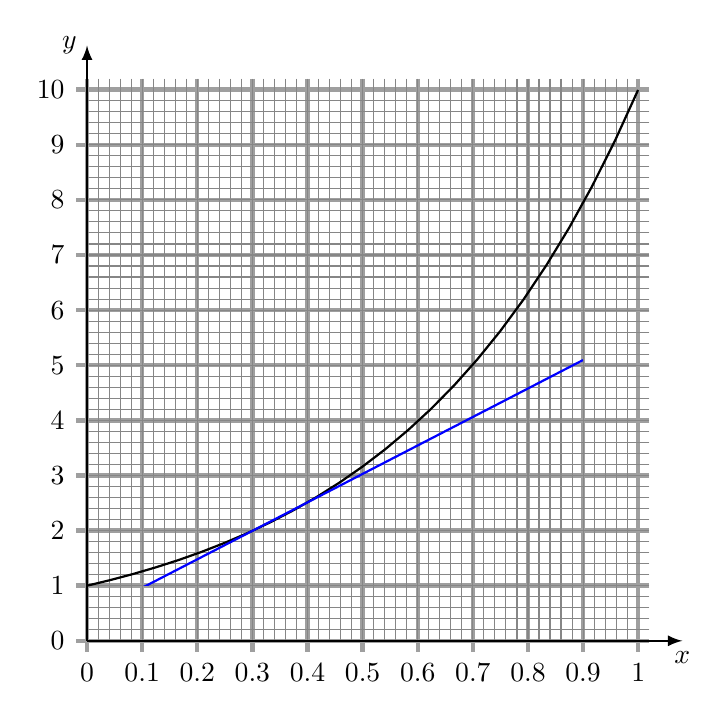
\begin{tikzpicture}[x=70mm,y=7mm,>=latex]
    \foreach \x in {0,0.1,0.2,0.3,0.4,0.5,0.6,0.7,0.8,0.9,1}
    {
      \draw[ultra thick,gray!75] (\x,10.2) -- (\x,-0.2) node[black,below] {$\x$};
    }
    \foreach \y in {0,1,...,10} 
    {
      \draw[ultra thick,gray!75] (1.02,\y) -- (-0.02,\y) node[black,left] {$\y$};
    }
    \foreach \k in {2,4,...,98}
    {
      \draw[thin,gray!95] ({\k/100},10.2) -- ({\k/100},0);
      \draw[thin,gray!95] (1.02,{\k/10}) -- (0,{\k/10});
    }
    %
    \draw[thick,black,->] (0,0) -- (1.08,0) node[below] {$x$};
    \draw[thick,black,->] (0,0) -- (0,10.8) node[left] {$y$};
    \draw[thick,black] plot[domain=0:1] (\x,{10^(\x)});
    % \node[black,fill=white] at (0.21,8.2) {$y=10^x$};
    \uncover<2->{%
      \begin{scope}
        \clip (0.1,1) rectangle (0.9,9);
        % y-10^0.3 = (10^0.3 - 10^0.2)/0.1 * ( x-0.3)
        \draw[thick,blue,domain=0.1:0.9] plot (\x,{10^(0.3)- (10^(1.3)-10^(1.4))*(\x-0.3)});
      \end{scope}
    }
  \end{tikzpicture}
  \bigskip

  % {\Large\textbf{Graph of $y=10^{x}$}}
  % \vspace*{0.5in}

  % \begin{tikzpicture}[x=30mm,y=3mm,>=latex,baseline=0,decoration={%
  %     markings,%
  %     mark=at position 0.55 with {\arrow[double,thick]{angle 60};}}%
  %     % mark=at position 0.6 with {\arrow{latex};}}%
  %   ]
  %   \draw[thick,black,->] (0,0) -- (1.08,0);% node[below] {$x$};
  %   \draw[thick,black,->] (0,0) -- (0,10.8);% node[left] {$y$};
  %   \draw[thick,black] plot[domain=0:1] (\x,{10^(\x)});
  %   \draw[thick,black] (0.8,{ln(0.8)/ln(10)}) -- (0.8,0);
  %   \node[left] at (0,{10^(0.8)}) {$\mbox{antilog}(x)$};
  %   \node[below] at (0.8,0) {$x$};
  %   \draw[thick,black,postaction=decorate] (0.8,{10^(0.8)}) -- (0,{10^(0.8)});
  %   \draw[thick,black,postaction=decorate] (0.8,0) -- (0.8,{10^(0.8)});
  % \end{tikzpicture}
  % \hspace*{1.5in}
  % \begin{tikzpicture}[x=30mm,y=3mm,>=latex,baseline=0,decoration={%
  %     markings,%
  %     mark=at position 0.55 with {\arrow[double,thick]{angle 60};}}%
  %     % mark=at position 0.6 with {\arrow{latex};}}%
  %   ]
  %   \draw[thick,black,->] (0,0) -- (1.08,0);% node[below] {$x$};
  %   \draw[thick,black,->] (0,0) -- (0,10.8);% node[left] {$y$};
  %   \draw[thick,black] plot[domain=0:1] (\x,{10^(\x)});
  %   \draw[thick,black,postaction=decorate] (0,{10^(0.8)}) -- (0.8,{10^(0.8)});
  %   \draw[thick,black,postaction=decorate] (0.8,{10^(0.8)}) -- (0.8,0);
  %   \node[left] at (0,{10^(0.8)}) {$y$};
  %   \node[below] at (0.8,0) {$\log(y)$};
  % \end{tikzpicture}

\end{center}


}



% \section{Interpretation of Derivatives}


% \frame{
%   \frametitle{Interpretation of Derivatives II}

%   Air temperature gets colder the higher you go.\\
%   $T({\red x})=$ {\blue air temperature} in $^{\circ}C$ at a height $\red x$ meters above sea level.

%   \alert{Question:}\ Which of these is a plausible value for $T'({\red 2000})$?
%   \begin{center}
%     A$ = -1$
%     \quad 
%     B$ = 1$
%     \quad 
%     C$ = 0$
%     \quad 
%     D$ = 1/200$
%     \quad 
%     E$ = -1/200$
%     \pause
%     \quad
%     \fbox{E} 
%   \end{center}
%   \pause
%   \gap 

%   \alert{Question:}\ If $T({\red 2000})={\purple 10}$ and $T{\red'}({\red 2000})=-{\bluegreen 1/200}$, which is most plausible?
%   \begin{itemize}
%   \item[A] the temperature at sea level is $16^oC$
%   \item[B] the temperature $2400$ meters above sea level is $8^oC$
%   \item[C] the temperature $10$ meters above sea level is $2000^oC$
%   \item[D] 2000 meters above sea level the temperature is decreasing at a rate of $1/200^oC$ per minute.
%   \item[E] none of these are plausible
%   \end{itemize}
%   \pause
%   \alert{Answer:}\ \fbox{B}


% }



% \frame{
%   \frametitle{Interpretation of Derivatives III}
%   \vspace*{-0.30in}

%   \begin{align*}
%     {\red x} 
%     & = \text{money spent (in thousands of \$) in one month on advertising.}\\
%     {\blue f(x)}
%     & = \text{{\blue sales} (in thousands of \$) in a month when ${\red x}$ is spent on advertising.}
%   \end{align*}
%   \pause\vspace*{-0.2in}

%   \alert{Question:}\ If $f({\red 20})={\blue 60}$ and $f{\red'}({\red 20})=3$ which must be true?
%   \begin{itemize}
%   \item[A] When the sales of the company are 20 thousand dollars in
%     one month the amount spent on advertising is increasing at a rate
%     of 3 thousand dollars per month

%   \item[B] When the company spends 20 thousand dollars per month on
%     advertising the sales rise at a rate of 3 thousand dollars per
%     month 
%   \item[C] When the company spends 20 thousand dollars per month on
%     advertising each extra dollar a month spent on advertising
%     generates an extra 3 dollars of sales. 

%   \item[D] When the company spends 3 thousand dollars per month on
%     advertising the sales are increasing at a rate of 20 thousand
%     dollars per month 

%   \item[E] None of the above
%     \pause
%     \hfill
%     \alert{Answer:}\ \fbox{C}
%   \end{itemize}

% }




\section{Linear Approximations}
\frame{
  \frametitle{\S8.6: Tangent Line Approximation}

  \alert{Question:}\ At 5am the temperature is $42^{\circ}\ \text{F}$ and increasing
  at a rate of $10^{\circ}\ \text{F}$ per hour. Which of the following do you think
  is closest to the temperature at 5:15am? 
  \begin{center}
    A$ = 2.5^{\circ}\ \text{F}$
    \quad 
    B$ = 52^{\circ}\ \text{F}$
    \quad 
    C$ = 43.5^{\circ}\ \text{F}$
    \quad 
    D$ = 44.5^{\circ}\ \text{F}$
    \quad 
    E$ =5.15^{\circ}\ \text{F}$
  \end{center}
  \pause
  \alert{Answer:}\ 
    \fbox{D}

    % \gap  5:15 is $1/4$ of an hour after 5am.\\
    % $\therefore\quad$ Temperature rises {\blue approximately} $(1/4)\times 10=2.5^{\circ}\ \text{F}$ in this time.\\
    % So final temperature is {\blue approximately} $42+2.5=44.5^{\circ}\ \text{F}.$

    % \gap
    % {\blue Approximately} because instantaneous rate of change is $10$ at $5am$ but this may change. Maybe by 5:10am temperature is increasing at a rate of $11^{\circ}\ \text{F}$ per hour.

    % \gap
    % Answer is \fbox{{\blue (initial temperature)} + {\red (rise in temperature)}}\\
    % {\red (rise in temperature)} $\approx$ (time taken) $\times$ {\green (rate of change)}
    
    % {\green rate of change} = {\green derivative}

    % \gap 
    % \includegraphics[scale=0.6]{inputoutput.pdf}

    \begin{center}
      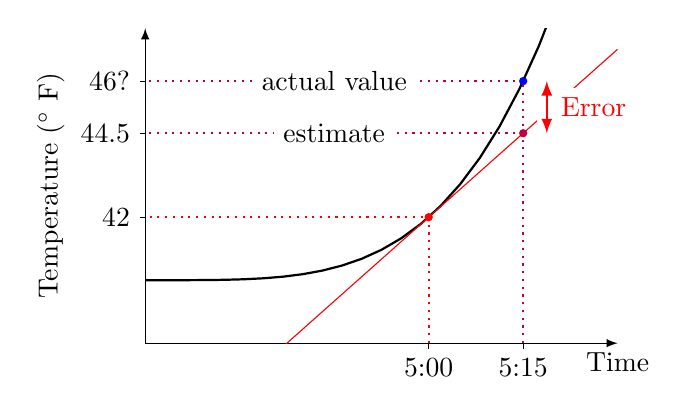
\begin{tikzpicture}[x=12mm,y=8mm,>=latex]
        \draw[thin,black,->] (0,0) -- (5,0) node[below] {Time};
        \draw[thin,black,->] (0,0) -- (0,5);
        \node[rotate=90] at (-1,2.5) {Temperature (${}^\circ\ \text{F}$)};
        \begin{scope}
          \clip (0,0) rectangle (5,5);
          \draw[thick,black,domain=0:5] plot (\x,{1+(\x/3)^4});
          % tangent line at (3,2) is y-2=(4/3)(x-3) or y=4x/3-2:
          \draw[thin,red,domain=0:5] plot (\x,{4*\x/3-2});
        \end{scope}
        \draw[black,thin] (3,0) -- (3,-2pt) node[below] {5:00};
        \draw[black,thin] (4,0) -- (4,-2pt) node[below] {5:15};
        \draw[black,thin] (0,2) -- (-2pt,2) node[left] {$42$};
        \draw[red,thick,dotted] (3,0) -- (3,2) -- (0,2);
        \fill[red] (3,2) circle (1.5pt);
        \fill[purple] (4,{4*4/3-2}) circle (1.5pt);
        \draw[thick,dotted,purple] (4,0) -- (4,{1+(4/3)^4});
        \draw[thick,dotted,purple] (4,{4*4/3-2}) -- (0,{4*4/3-2}) node[midway,black,fill=white] {estimate};
        \draw[black,thin] (0,{4*4/3-2}) -- (-2pt,{4*4/3-2}) node[left] {$44.5$};
        \draw[thick,dotted,purple] (4,{1+(4/3)^4}) -- (0,{1+(4/3)^4}) node[midway,black,fill=white] {actual value};
        \draw[black,thin] (0,{1+(4/3)^4}) -- (-2pt,{1+(4/3)^4}) node[left] {$46$?};
        \fill[blue] (4,{1+(4/3)^4}) circle (1.5pt);
        \filldraw[white] (4.15,{4*4/3-2-0.5}) rectangle (4.5,{1+(4/3)^4+0.25});
        \draw[red,thick,fill=white,<->] (4.25,{4*4/3-2}) -- (4.25,{1+(4/3)^4}) node[midway,right,red,fill=white,xshift=0.5mm] {Error};
      \end{tikzpicture}
    \end{center}
  
}



\frame{
  \frametitle{Continuing this example}
  
  Same set-up:
  \begin{itemize}
  \item $f({\red x})=$ temperature at {\red time $x$}\ hours after midnight

  \item $f(5)=42$ ($42^{\circ}\ \text{F}$ at 5:00am)

  \item $f{\red'}(5)=2$
  \end{itemize}

  \alert{(1)}\ Find the equation of {\blue tangent line} to $y=f(x)$ at $x=5$.

  \begin{center}
    A\ \ $y = 5x+42$
    \qquad
    B\ \ $y = 2x+5$
    \qquad
    C\ \ $y = 2(x-5)+42$
    \\
    D \ \  $y -5 = 2(x-42)$ 
    \qquad
    E \ \  $y -42 = 2x-5$ 
  \end{center}
  \pause
  \alert{Answer:}\ \fbox{C}
  \pause

  \alert{(2)}\ Use this to predict the approximate temperature at 4am.
  \begin{center}
    A$ = 40$
    \quad 
    B$ = 41$
    \quad 
    C$ = 42$
    \quad 
    D$ = 43$
    \quad 
    E$ = 44$
    \pause
    \quad
    \fbox{A}
  \end{center}
  \pause

  \alert{(3)}\ The tangent line approximation is used to estimate the
  temperature at the following times. Which do you think is most
  accurate?
  \begin{center}
    A\ 4am
    \quad 
    B\ 4:50am
    \quad 
    C\ 5:25am
    \quad 
    D\ 6am
    \quad 
    E\ midnight
    \quad
    \pause
    \fbox{B}
  \end{center}

}


\frame{
  \frametitle{Tangent Line Approximation}

  To do a tangent line approximation:
  \begin{itemize}
  \item[(i)] Find the equation of the tangent line.

  \item[(ii)] Plug in the required value(s) into this equation.

  \end{itemize}
  \gap

  Suppose $f({\orange 4})={\blue 2}$ and $f{\red'}({\orange 4})={\red 3}$.

  \begin{itemize}
  \item[\red(a)]  The equation of the tangent line to $y=f(x)$ at $x={\orange 4}$ is $y=$?
    \begin{center}
      A$ = {\orange 4}x-{\purple 14}$
      \qquad 
      B$= {\orange 3}x-{\purple 10}$
      \qquad 
      C$= {\orange 2}x-{\purple 6}$
      \\
      \ \hfill
      D$={\orange 3}x-{\purple 4}$
      \qquad 
      E$= {\orange 2}x-{\purple 5}$
      \pause 
      \hfill
      \fbox{B}
    \end{center}
    \pause

  \item[\red(b)] Use this tangent line approximation to estimate $f(4.1)$.
    \begin{center}
      A$=2.3$
      \quad 
      B$= 1.7$
      \quad 
      C$ = 2.6$
      \quad 
      D$ = 1.4$
      \quad 
      E$ = 2$
      \pause
      \quad
      \fbox{A}
    \end{center}


  \item[\red(c)]
    Use the tangent line approximation to estimate the value of $x$ which gives $f(x)=2.9$.
    \begin{center}
      A$ = 4.9$
      \quad 
      B$ = 4.1$
      \quad 
      C$ = 2.9$
      \quad 
      D$ = 4.1$
      \quad 
      E$ = 4.3$
      \pause
      \quad
      \fbox{E}
    \end{center}
  \end{itemize}

}

\frame{
  \frametitle{Standard Estimation Problem}

  \alert{Question:}\ Approximate $\sqrt{26}$.

  \begin{center}
    A$=0.1$
    \quad 
    B$= 5.01$
    \quad 
    C$ = 5.05$
    \quad 
    D$ = 5.1$
    \quad 
    E$ = 5.2$
    \quad
    \uncover<3->{\fbox{D}}
  \end{center}

  \uncover<2->{%
    \alert{Hint:}\ If $g(x)=\sqrt{x}$, then $g{\red'}({\blue 25})={\red
      1/10}$ and $g({\blue25}) = \sqrt{\blue 25}={\bluegreen 5}$.
  }
  \gap
  \gap

  \uncover<4->{%
    \alert{Better estimate:}\ $\sqrt{26}\approx5.09902$, so the {\red
      error} in the tangent line approximation here is
    \begin{equation*}
      \text{\red{}error} 
      \approx 5.1-5.09902
      \approx0.001
    \end{equation*}
    This is a percentage error of only $\red 0.02\%$.
  }

}


\frame{
  \frametitle{Another Example:}

  \begin{itemize}
  \item $f(t) = \text{number of grams of a chemical reagent after $t$
      seconds}$
    \smallskip

  \item We're told $f(0)=20$ and $f{\red'}(0)=-3$
    \smallskip
  \end{itemize}

  \alert{Question:}\ Roughly how many grams are there after $t$ seconds?

  \begin{center}
    A$=4-3t$
    \quad 
    B$= 20-3t$
    \quad 
    C$ = 20-4t$
    \quad 
    D$ =20 + 4t$
    \quad 
    E$ = 32-3t$
  \end{center}
  \pause

  \alert{Answer:}\ \fbox{B}


}


\frame{
  \frametitle{Lake Cachuma {\small(a linear approximation)}}
  % From {\red http://www.montecitowater.com/Sources_of_water.htm}
  \begin{itemize}
  \item Lake Cachuma was completed in 195{\red 0}.  \hfill{ \it
      \tiny{really completed 195{\red 3}}}

  \item It originally had a capacity of 205,000 acre feet ({\blue this
      is volume}). 

  \item In 2010 it has a capacity of approximately 190,000 acre-feet
    as a result of the accumulation of silt in the reservoir.

  \item ${\blue f(t)} = \text{{\blue{}capacity} in acre-feet of
      Cachuma lake $t$ years after 195{\red 0}}$. 
  \end{itemize}
  \gap

  \alert{(1)}\ Write down a linear approximation from this
  information for $\blue f(t)$. 
  \begin{center}
    A$ = 205,000-15,000t$
    \quad 
    B$ = 190,000+250t$
    \quad 
    C$ = 205,000-250t$\\[0.5em]
    %
    \ \quad
    D$ = 190,000-250t$
    \quad
    E$ = 190,000-125t$
    \quad
    \pause
    \fbox{C}
  \end{center}
  \vspace{.05in} 

  % Change in volume is $190000-205000=-15000.$ Change in time is
  % $2010-1950=60$ years. Average rate of change = $-15000/60=-250.$ So
  % Linear approximation is $f(t)=-250t+{\red b}.$ But
  % $f(0)=205000={\red b}.$ So \fbox{$f(t)=205000-250t$}
  % \vspace{.05in} 

  \alert{(2)}\ Which of the following years is the best
  estimate for when $10\%$\ of its original capacity will have been
  lost due to silt?
  \begin{center}
    A$= 2027$
    \quad 
    B$ = 2032$
    \quad 
    C$ = 2037$
    \quad 
    D$ = 2042$
    \quad 
    E$ = 2047$
    \pause
    \quad
    \fbox{B}
  \end{center}

}

\end{document}
\section{Sketching Curves}

\frame{
  \frametitle{Sketching some simple graphs}

  It's useful to be able to sketch\ldots
  \smallskip

  \alert{(1)\ Quadratics}

  \begin{minipage}{0.45\linewidth}
    \begin{center}
      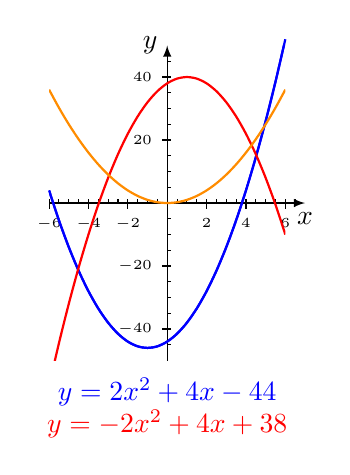
\begin{tikzpicture}[x=2.5mm,y=0.4mm,>=latex]
        \draw[thin,black,->] (-6,0) -- (7,0) node[below] {$x$};
        \draw[thin,black,->] (0,-50) -- (0,50) node[left] {$y$};
        % ticks:
        \foreach \x in {-6,-4,-2,2,4,6}
        {
          \draw[thin,black] (\x,0) -- (\x,-2pt) node[below] {$\scriptscriptstyle\x$};
        }
        \foreach \x in {-6,-5.5,...,6.5}
        {
          \draw[thin,black] (\x,0) -- (\x,1.5pt);
        }
        \foreach \y in {-40,-20,20,40}
        {
          \draw[thin,black] (0,\y) -- (-2pt,\y) node[left] {$\scriptscriptstyle\y$};
        }
        \foreach \y in {-45,-40,...,45}
        {
          \draw[thin,black] (0,\y) -- (1.5pt,\y);
        }
        \draw[thick,blue,domain=-6:6,smooth] plot (\x,{2*(\x)^2+4*\x-44});
        % graphs:
        \begin{scope}
          \clip (-6,-50) rectangle (6,50);
          \draw[thick,blue,domain=-6:6,smooth] plot (\x,{2*(\x)^2+4*\x-44});
          \draw[thick,red,domain=-6:6,smooth] plot (\x,{-2*(\x)^2+4*\x+38});
          \uncover<2->{%
            \draw[thick,orange!90!yellow,domain=-6:6,smooth] plot (\x,{(\x)^2});
          }
        \end{scope}
        % labels:
        \node[blue] at (0,-60) {$y=2x^2+4x-44$};
        \node[red] at (0,-70) {$y=-2x^2+4x+38$};
      \end{tikzpicture}
    \end{center}
  \end{minipage}
  \hfill
  \begin{minipage}{0.5\linewidth}
    \begin{itemize}
    \item $y=ax^2+bx+c$
    \item Bowl-shaped:
      \begin{itemize}
      \item[\red$\star$] Opens up if $a>0$
      \item[\red$\star$] Opens down if $a<0$
      \end{itemize}
    \item Model curve: $y=x^2$ \\
      \uncover<2->{\colorbox{blue!25}{\color{orange!90!yellow}Shown here!}}
    \end{itemize}
  \end{minipage}
  \vspace*{2in}

}

\frame{
  \frametitle{Sketching some simple graphs}


  It's useful to be able to sketch\ldots
  \smallskip

  \alert{(2)\ Cubics}

  \begin{minipage}{0.45\linewidth}
    \begin{center}
      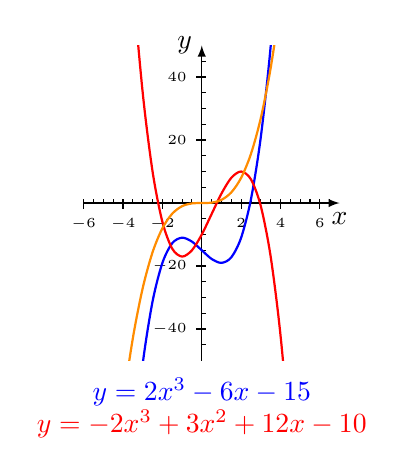
\begin{tikzpicture}[x=2.5mm,y=0.4mm,>=latex]
        \draw[thin,black,->] (-6,0) -- (7,0) node[below] {$x$};
        \draw[thin,black,->] (0,-50) -- (0,50) node[left] {$y$};
        % ticks:
        \foreach \x in {-6,-4,-2,2,4,6}
        {
          \draw[thin,black] (\x,0) -- (\x,-2pt) node[below] {$\scriptscriptstyle\x$};
        }
        \foreach \x in {-6,-5.5,...,6.5}
        {
          \draw[thin,black] (\x,0) -- (\x,1.5pt);
        }
        \foreach \y in {-40,-20,20,40}
        {
          \draw[thin,black] (0,\y) -- (-2pt,\y) node[left] {$\scriptscriptstyle\y$};
        }
        \foreach \y in {-45,-40,...,45}
        {
          \draw[thin,black] (0,\y) -- (1.5pt,\y);
        }
        % graphs:
        \begin{scope}
          \clip (-6,-50) rectangle (6,50);
          \draw[thick,blue,domain=-6:6,smooth] plot (\x,{2*(\x)^3-6*\x-15});
          \draw[thick,red,domain=-6:6,smooth] plot (\x,{-2*(\x)^3+3*(\x)^2+12*\x-10});
          \uncover<2->{%
            \draw[thick,orange!90!yellow,domain=-6:6,smooth] plot (\x,{(\x)^3});
          }
        \end{scope}
        % labels:
        \node[blue] at (0,-60) {$y=2x^3-6x-15$};
        \node[red] at (0,-70) {$y=-2x^3+3x^2+12x-10$};
      \end{tikzpicture}
    \end{center}
  \end{minipage}
  \hfill
  \begin{minipage}{0.5\linewidth}
    \begin{itemize}
    \item $y=ax^3+bx^2+cx+d$
    \item ``S''-shaped:
      \begin{itemize}
      \item[\red$\star$] Goes to $+\infty$ if $a>0$
      \item[\red$\star$] Goes to $-\infty$ if $a<0$
      \end{itemize}
    \item Model curve: $y=x^3$ \\
      \uncover<2->{\colorbox{blue!25}{\color{orange!90!yellow}Shown here!}}
    \end{itemize}
  \end{minipage}
  \smallskip
  \uncover<3->{%
    \begin{empheq}[box=\othermathbox]{align*}
      \text{For a polynomial, the {\blue highest power}\ of $x$ {\red dominates}\ when $x$ is big}    
    \end{empheq}
  }
  \vspace*{2in}



}

\section{Computing Derivatives}

\frame{
  \frametitle{The Derivatives of Simple Functions}

  \begin{minipage}{0.45\linewidth}
    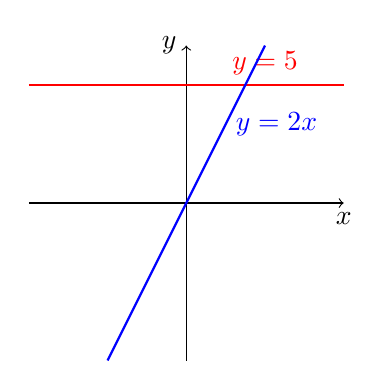
\begin{tikzpicture}
      \draw[thin,black,->] (-2,0) -- (2,0) node[below] {$x$};
      \draw[thin,black,->] (0,-2) -- (0,2) node[left] {$y$};
      \uncover<1-4>{%
        \draw[thick,red] (-2,1.5) -- (2,1.5) node[near end,above] {$y=5$};
      }
      \uncover<5->{%
        \draw[thick,blue] (-1,-2) -- (1,2) node[near end,right] {$y=2x$};
      }
    \end{tikzpicture}
  \end{minipage}
  \hfill
  \begin{minipage}{0.52\linewidth}
    The derivative of a constant is\only<1>{\ldots?}%
    \uncover<2->{%
      \ zero because:
       \begin{itemize}
       \item {\red$\text{derivative} = \text{rate of change}$}
       \item {\red constants don't change}\\[0.5em]
         \uncover<3->{%
       \item {\blue$\text{derivative} = \text{slope}$}
       \item {\blue$\text{slope} = 0$}
         }
       \end{itemize}
      \uncover<4->{So $\dfrac{d}{dx} \big( 5 \big) = 0$}
     }
  \end{minipage}
  \medskip

  \uncover<5->{%
    The derivative of a straight line is\only<5>{\ldots?}}\only<6->{%
    \ its slope because}
  \uncover<6->{%
    \begin{itemize}
    \item {\blue$\text{derivative} = \text{slope}$}
    \end{itemize}
  }
  \uncover<7->{So $\dfrac{d}{dx}\big(2x\big) = 2$}

}


\frame{
  \frametitle{Meaning of Derivatives}

  \begin{minipage}{0.45\linewidth}
    \begin{empheq}[box=\othermathbox]{align*}
      \Large%
      \frac{d}{dx}\left( x^2\right) = 2x      
    \end{empheq}
    % \vspace{.1in}

    What this {\blue means}
    %% \vspace{.1in}

    \begin{empheq}[box=\othermathbox]{align*}
      \text{The {\red slope} of the graph\ }\\
      \text{of ${\blue y=x^2}$ at $x={\red a}$ is $2{\red a}$}
    \end{empheq}
  \end{minipage}
  \hspace*{0.25in}
  \begin{minipage}{0.45\linewidth}
    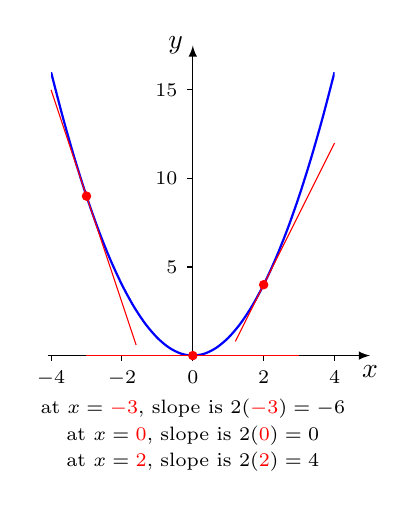
\begin{tikzpicture}[x=4.5mm,y=2.25mm,>=latex]
      \draw[thin,black,->] (-4.1,0) -- (5,0) node[below] {$x$};
      \draw[thin,black,->] (0,0) -- (0,17.5) node[left] {$y$};
      % ticks:
      \foreach \x in {-4,-2,0,2,4}
      {
        \draw[thin,black] (\x,0) -- (\x,-2pt) node[below] {$\scriptstyle\x$};
      }
      \foreach \y in {5,10,15}
      {
        \draw[thin,black] (0,\y) -- (-2pt,\y) node[left] {$\scriptstyle\y$};
      }
      \begin{scope}
        \clip (-4,0) rectangle (4,16);
        \draw[blue,thick,domain=-4:4,smooth] plot (\x,{(\x)^2});
      \end{scope}
      \uncover<2>{%
        \node at (0,-3) {$\scriptstyle\text{at $x={\red-3}$, slope is $2({\red-3})=-6$}$};
        % tangent line is y-9=-6(x+3) or y=-6x-9
        \draw[thin,red,domain=-4:-1.6] plot (\x,{-6*\x - 9});
        \filldraw[red] (-3,9) circle (1.5pt);
      };
      \uncover<3>{%
        \node at (0,-4.5) {$\scriptstyle\text{at $x={\red0}$, slope is $2({\red0})=0$}$};
        % tangent line is y=0
        \draw[thin,red] (-3,0) -- (3,0);
        \filldraw[red] (0,0) circle (1.5pt);
      };
      \uncover<4->{%
        \node at (0,-6) {$\scriptstyle\text{at $x={\red2}$, slope is $2({\red2})=4$}$};
        % tangent line is y-4=4(x-2) or y=4x-4
        \draw[thin,red,domain=1.2:4] plot (\x,{4*\x - 4});
        \filldraw[red] (2,4) circle (1.5pt);
      };
    \end{tikzpicture}
  \end{minipage}
  % \gap

  \uncover<5->{%
    \begin{empheq}[box=\othermathbox]{align*}
      \text{derivative}
      = \text{rate of change}
      = \text{slope of graph}
      = \text{slope of tangent line}
    \end{empheq}
  }



}



\frame{
  \frametitle{General Rule:}

  \begin{minipage}{0.45\linewidth}
    \begin{align*}
      \frac{d}{dx}\left(x^{\red 2}\right) & = {\red 2}x\\
      \frac{d}{dx}\left(x^{\red 3}\right) & = {\red 3}x^{\blue 2}\\
      \frac{d}{dx}\left(x^{\red 4}\right) & = {\red 4}x^{\blue 3}
    \end{align*}
  \end{minipage}
  \begin{minipage}{0.45\linewidth}
    \uncover<2->{%
      \begin{empheq}[box=\othermathbox]{align*}
        \frac{d}{dx}\left(x^{\red n}\right) & = {\red n}x^{\blue n-1}
      \end{empheq}
    }
  \end{minipage}
  \smallskip
  
  \uncover<3->{%
    The {\red exponent} comes out front. Then {\blue subtract} one
    from exponent.
  }

  \uncover<4->{\alert{Examples:}}
  \pause\pause\pause\pause

  {\red(1)} $\dfrac{d}{dx}\left( x^{\red 7}\right) = $
  \begin{center}
    A$ = 7x^7$
    \quad 
    B$ = 6x^6$
    \quad 
    C$ = 6x^7$
    \quad 
    D$ = 7x^6$
    \quad 
    E$ = 0$
    \quad
    \pause
    \fbox{D}
  \end{center}

  {\red(2)} $\dfrac{d}{dx}\left( x^{\red -3}\right) = $
  \begin{center}
    A$ = 3x^{-2}$
    \quad 
    B$ = -3x^{-2}$
    \quad 
    C$ = -2x^{-4}$
    \quad 
    D$ = -3x^{-4}$
    \quad
    \pause
    \fbox{D}
  \end{center}
}

\frame{
  \frametitle{More Examples}
  \begin{empheq}[box=\othermathbox]{align*}
    \frac{d}{dx}\left(x^{\red n}\right) & = {\red n}x^{\blue n-1}
  \end{empheq}

  {\red(3)} $\dfrac{d}{dx}\left( x^{\red 1/2}\right) = $
  \begin{center}
    A$ = \frac{1}{2}x^{1/2}$
    \quad 
    B$ = -\frac{1}{2}x^{-1/2}$
    \quad 
    C$ =  \frac{1}{2}x^{-1/2}$
    \quad
    \pause
    \fbox{C}
  \end{center}
  \pause

  \alert{Rule:}\ {\red ALWAYS}\  {\blue re}write {\blue the
    thing} you want derivative of  as $x^{\red n}$
  \pause\smallskip

  {\red(4)} $\dfrac{d}{dx}\left( {\frac{1}{x^3}}\right) = $
  \begin{center}
    A$ = \frac{1}{3x^2}$
    \quad 
    B$ = -3x^{-2}$
    \quad 
    C$ = -3x^{-4}$
    \quad
    \pause
    \fbox{C}
  \end{center}
  \pause

  {\red(5)} $\dfrac{d}{dx}\left({\sqrt{x}}\right) = $
  \begin{center}
    A$ =-\frac{1}{2}\sqrt{x}$
    \quad 
    B$ = \frac{1}{2}{x}^{-1/2}$
    \quad 
    C$ =  -\frac{1}{2}{x}^{-1/2}$
    \quad
    \pause
    \fbox{B}
  \end{center}


}


\end{document}
\frame{

\includegraphics[scale=0.8]{field.pdf}

A field has area 5000 square meters. It is surrounded by a wood fence that costs \$6 per meter length. It is divided in half by a brick wall that costs \$15 per meter length. Express the total costs of the wall and fence in terms of  $x=$ length of the wall in meters.

\gap
$A = 5000x\quad B = 15x+12W\quad C = 27x + 60000/x$\\
$ D = 15x + 30000/x\quad E = {\red hint}$\pause\\
Draw a {\red PLP} ={\red P}retty {\red L}ittle {\red P}icture\\
Name (and label on {\red PLP}) unknowns (length, width )\\
Get formula for {\blue cost} ({\purple of what exactly ?}) in terms of length and width\\
use given information to eliminate the dimension you don't want.




}

\frame{

\includegraphics[scale=0.8]{field2.pdf}

A field has area 5000 square meters. It is surrounded by a wood fence that costs \$6 per meter length. It is divided in half by a brick wall that costs \$15 per meter length. Express the total costs of the wall and fence in terms of  $x=$ length of the wall in meters.

\gap
$A = 5000x\quad B = 15x+12W\quad C = 27x + 60000/x$\\
$ D = 15x + 30000/x$\quad\fbox{\blue C}

\gap $W=$ length of side of field perpendicular to brick wall.\\
$C=$ total cost =(cost brick)+(cost fence) \\
(cost brick) $=15x$\qquad (cost fence)=$6(2x+2W)=12x+12W$\\
$\therefore\quad C=15x+(12x+12)=27x+12W$\\
Area of field $=5000=xW$ so $W=5000/x.$\\
 Substitute for $W$ in above get $C=27x+12(5000/x)=27x+60000/x$


}

\frame{

An airline normally sells 3000  tickets per week on a certain route for \$200. When it has a sale, for every \$5 the price is lowered the number of tickets sold on the route increases by 60. Suppose the price is reduced by $5n$ dollars to \$(200-5n). How many tickets are sold ?\\
$A = 3000\quad B = 60\times (200-5n)\quad C =3000+(200-5n)\times 60$\\
$D = 3000+60n\quad E = 3000+12n$\pause\quad\fbox{\blue D}

\gap Reducing price \$$5n$ increases number of tickets by $60n$ to give total number of tickets = \fbox{$3000+60n$}

\gap If the ticket price is \$x how many tickets are sold?\\
$A = 3000-12x\quad B = 3000-60(200-x)\quad C = 5400-12x $\\
$ D = 3000+12x\quad E = 600+12x$\pause\quad\fbox{\blue C}

\gap $x=200-5n.$ Solve for $x$ get $5n=200-x$ so $n=40-(x/5).$\\
Substitute into $3000+60n$ for $n$ get $3000+60(40-(x/5))=$\fbox{$5400-12x$}

}








\frame{

{\blue HW18} {\it In the year 1900, in the country Acirema, there were {\blue 100} Lawyers and 
3 million people. Every {\red 10} years, the number of Lawyers doubles, and the population 
increases by 2 million. Let {\green t} be the number of years after 1900. Thus t=3 corresponds 
to 1903. Find the equation involving {\green t} whose solution tells you in which year 20 percent 
of the population are Lawyers. }

\gap $L({\green t}) =$ number of lawyers after ${\green t}$ years\\
$P({\green t}) = $ number of people after ${\green t}$ years\\

\halfgap Told initial population is 3 million and increases by 2 million in 10 years\\
 so increases 200,000 in 1 year so\qquad
$P({\green t})=3,000,000+200,000{\green t}$\halfgap

Told doubling time for lawyers is ${\red K}=\red 10$ years\\ 
{\blue initial number} is {\blue 100} so\qquad\qquad\qquad
$L({\green t})={\blue 100}\times2^{{\green t}/\red 10}$\\
Have 20\% Lawyers when
$$\frac{L({\green t})}{P({\green t})}=0.2=\frac{{\blue 100}\times2^{{\green t}/\red 10}}{(3,000,000+200,000{\green t})}$$


}





  
\end{minipage}